\documentclass[../main.tex]{subfiles}

\begin{document}
%%%%%%%%%%%%%%%%%%%%%%%%%%%%%%%%%%%%%%%%%%%%%%
%                                            %
% PoMehrdimensionale Differentialrechnung II %
%                                            %
%%%%%%%%%%%%%%%%%%%%%%%%%%%%%%%%%%%%%%%%%%%%%%
\chapter{SW14 Mehrdimensionale Differentialrechnung II}
\section{Totales Differential}
"Komplete" Ableitung von Funktion mit mehreren Variablen $f(x,y)$: \\ [7pt]
$df=f_x(a,b)dx+f_y(a,b)dy$ oder in Kurzform $df=f_xdx+f_ydy$

\section{Linearisierung von Funktionen}
\subsection{...mit einer Variable}
$f(x)$,$t(x)$ ist die Linearisierung (Tangente), $x_0$ 
ist der Punkt wo linearisiert wird/Tangente anliegt \\ [7pt]
$t(x)=mx + b$ oder $t(x)=f(x_0) + f'(x)(x-x_0) = f(x_0)+f'(x_0)\cdot x-f'(x_0)\cdot x_0$ \\
$m=f'(x_0)$ \\
$b=f(x_0)-f'(x_0)\cdot x_0$

\subsection{...mit mehrern Variablen}
$g(x,y)$ \\ [7pt]
$L(x,y)=g(x_0,y_0)+g_x(x_0,y_0)(x-x_0)+g_y(x_0,y_0)(y-y_0)$ \\ [7pt]
$\nabla g(x_0,y_0)=\begin{pmatrix}g_x(x_0,y_0)\\g_y(x_0,y_0)\end{pmatrix}$ \\ [7pt]
$L(x,y)=g(x_0,y_0) + \nabla g(x_0,y_0) \cdot \begin{pmatrix}x-x_0\\y-y_0\end{pmatrix}$ \\ [14pt]
\noindent\rule{8cm}{0.4pt} \\
$h(x,y,z)$ \\ [7pt]
$\nabla h(x_0,y_0,z_0) = \begin{pmatrix}h_x(x_0,y_0,z_0)\\h_y(x_0,y_0,z_0)\\h_z(x_0,y_0,z_0)\end{pmatrix}$ \\ [7pt]
$M(x,y,z) = h(x_0,y_0,z_0)+ \nabla h(x_0,y_0,z_0) \cdot \begin{pmatrix}x-x_0\\y-y_0\\z-z_0\end{pmatrix}$

\section{Tangente an die Konturlinie}
$f(x,y)$ \\
$p(x_0,y_0)$ \\ [7pt]
Gleichung der Tangente an die Konturlinie von $f$ im Punkt $p$ ist: \\ [7pt]
$f_x(x_0,y_0)(x-x_0)+f_y(x_0,y_0)(y-y_0) = 0$

\section{Tangentialebene an die Konturfläche}
$f(x,y,z)$ \\
$p(x_0,y_0,z_0)$ \\ [7pt]
Gleichung der Tangentialebene an die Konturfläche: \\ [7pt]
$f_x(x_0,y_0,z_0)(x-x_0)+f_y(x_0,y_0,z_0)(y-y_0)+f_z(x_0,y_0,z_0)(z-z_0)=0$

\section{Newton-Raphson Methode}
Wir wollen die nichtlineare Gleichung $f(x)=0$ lösen. \\
Startpunkt: $x_n$ \\ [7pt]
$x_n - \frac{f(x_n)}{f'(x_n)}=x_{n+1}$ \\ [7pt]
Prozess beliebig wiederholen mit $x_{n+1}$ etc, bis man Nullstelle gefunden hat.

\section{Mehrdimensionale Newton-Raphson Methode}
Wird eher nicht an der Prüfung kommen.

\section{Kettenregel}
Falls $f,g,h$ differenzierbar sind und falls $z=f(x,y)$, $x=g(t)$, $y=h(t)$, dann ist die Ableitung
von $f$ nach $t$: \\ [7pt]
$f(x,y)$ \\ [7pt]
$\frac{df}{dt} = \frac{\partial f}{\partial x} \cdot \frac{dx}{dt}$
$+\frac{\partial f}{\partial y}\cdot\frac{dy}{dt}$

\subsection{Beispiel}
Sei $z=f(x,y)=x\sin y$, wobei $x=t^2$ und $x=t^2$. Sei $z=\bar{f}(t)=f(x(t),y(t))$.
Berechnen sie $\bar{f}'(t)$ einerseits direkt und anderseits mit der Kettenregel. \\ [7pt]
$f(x,y)=x\sin y$ \\[7pt]
$x=t^2$\\[7pt]
$x=t^2$\\[7pt]
\textbf{Direkt (Produkt- und Kettenregl):}\\[7pt]
$f(x(t),y(t))=x(t)\sin(y(t)) = t^2(\sin(2t+1))$ \\ [7pt]
$\frac{df}{dt}=2t\sin(2t+1)+t^2\cos(2t+1)\cdot 2$ \\ [7pt]
\textbf{Kettenregel:}\\[7pt]
$\frac{df}{dt} = \frac{\partial f}{\partial x} \cdot \frac{dx}{dt}$
$+\frac{\partial f}{\partial y}\cdot\frac{dy}{dt}$ \\ [7pt]
$\frac{\partial f}{\partial x}=\sin y$ \\ [7pt] 
$\frac{\partial f}{\partial y}= x \cos y$ \\ [7pt]
$\frac{dx}{dt}=x'(t)=2t$ \\ [7pt]
$\frac{dy}{dt}=y'(t)=2$ \\ [7pt]
$\frac{df}{dt} = \sin(2t+1)\cdot 2t + t^2\cos(2t+1)\cdot 2$

\section{Kettenregel mit Abhängigkeitsgraphen}
Um die partielle Ableitung einer zusammengesetzten Funktion mit mehreren Variablen zu berechnen, 
hilft der Abhängigkeitsgraph, welcher aufzeigt, wie die Variablen voneineander abhängen. \\
\begin{minipage}{0.45\textwidth}
    \begin{itemize}
        \item Zeichne einen Graphen, in welchem die Beziehungen zwischen den Variablen ersichtlich werden.
        Knoten sind die Variablen und auf den Kanten wird die entsprechende partielle Ableitung eingetragen.
        \item Für jeden Pfad zwischen zwei Variablen werden die partiellen Ableitungen auf den Kanten multipliziert.
        \item Dann werden die Beträge der jeweiligen Pfaden addiert.
    \end{itemize}
\end{minipage} \hfill
\begin{minipage}{0.5\textwidth}
    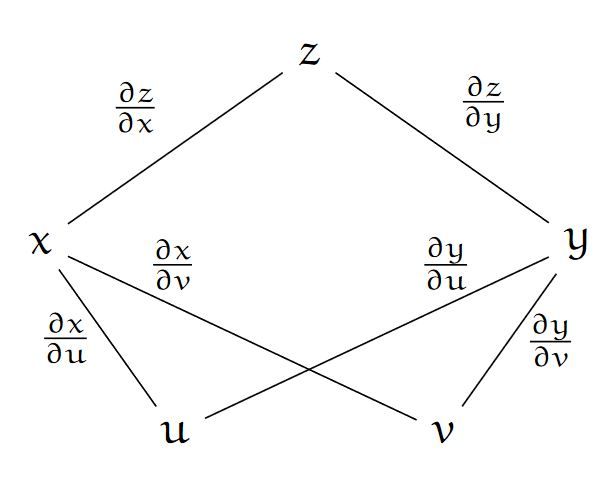
\includegraphics[width=50mm,scale=0.5]{abhaengigkeitsgraph}
\end{minipage}
\\ [7pt]
Falls $f,g,h$ differenzierbar sind und falls $z=f(x,y),x=g(u,v),y=(u,v)$, dann gilt: \\ [7pt]
$\frac{\partial z}{\partial u} = \frac{\partial z}{\partial x} \cdot \frac{\partial x}{\partial u}$
$+ \frac{\partial z}{\partial y} \cdot \frac{\partial y}{\partial u}$ und
$\frac{\partial z}{\partial v} = \frac{\partial z}{\partial x} \cdot \frac{\partial x}{\partial v}$
$+ \frac{\partial z}{\partial y} \cdot \frac{\partial y}{\partial v}$

\subsection{Beispiel}
$z=x^2e^y$ \\
$x=4u$ \\
$y=3u^2-2v$ \\ [7pt]
$\frac{\partial z}{\partial u} = \frac{\partial z}{\partial x}\frac{\partial x}{\partial u}+\frac{\partial z}{\partial y}\frac{\partial y}{\partial u}$ \\[7pt]
$=2xe^y\cdot 4 + x^2e^y\cdot 6u = 8xe^y+6ux^2e^y=2xe^y(4+3ux)$
$=2\cdot 4u \cdot e^{3u^2-2v}(4+3u\cdot 4u)=8ue^{3u^2-2v}(4+12u^2)$
$=32ue^{3u^2-2v}(1+3u^2)$ \\ [7pt]
$zv$ gleich berechnen!


\section{Kritische Punkte Beispiel}
$f(x,y)=\frac{1}{4}(x^4-2x^2+y^4-2y^2)$\\ [7pt]
$\nabla f=\begin{pmatrix}x^3-x\\y^3-y\end{pmatrix}$ Kritische Punkte: $\nabla f=0$ \\ [7pt]
$I: x^3-x = x(x^2-1) = 0 \longrightarrow x=0;x=1;x=-1$ \\ [7pt]
$II: y^3-y = y(y^2-1) = 0 \longrightarrow y=0;y=1;y=-1$ \\ [7pt]
$x$ und $y$ wild kombinieren für alle kritischen Punkte!

\section{Partielle Ableitungen zweiter Ordnung}
Die partiellen Ableitungen einer Funktion sind meist wieder Funktionen und können deshalb wieder abgeleitet werden. Dadurch
entstehen die zweiten partiellen Ableitungen oder die partiellen Ableitungen 2. Ordnung. Diesen Prozess kann man natürlich
wiederholen! \\ [7pt]
Die partiellen Ableitungen zweiter Ordnung von $z=f(x,y)$ \\ [7pt]
$\frac{\partial}{\partial x}(\frac{\partial f}{\partial x})=\frac{\partial^2z}{\partial x^2} = f_{xx} = (f_x)_x$ \\ [7pt]
$\frac{\partial}{\partial y}(\frac{\partial f}{\partial y})=\frac{\partial^2z}{\partial y^2} = f_{yy} = (f_y)_y$ \\ [7pt]
$\frac{\partial}{\partial y}(\frac{\partial f}{\partial x})=\frac{\partial^2z}{\partial y\partial x} = f_{xy} = (f_x)_y$ \\ [7pt]
$\frac{\partial}{\partial x}(\frac{\partial f}{\partial y})=\frac{\partial^2z}{\partial x\partial y} = f_{yx} = (f_y)_x$ \\ [7pt]
Die partiellen Ableitungen zweiter Ordnung haben etwas mit der \textbf{Krümmung} der Funktion zu tun.


\subsection{Beispiel}
$f(x,y)=xy^2+3x^2e^y$ \\ [7pt]
$f_x=y^2+6xe^y$ \\ [7pt]
$f_{xx}=6e^y$ \\ [7pt]
$f_{xy}=2y+6xe^y$ \\ [7pt]
$f_y=2xy+3x^2e^y$ \\ [7pt]
$f_{yy}=2x+3x^2e^y$ \\ [7pt]
$f_{yx}=2y+6xe^y = f_{xy}$ 

\section{Klassifikation kritischer Punkte - Theorem}
Die Funktion $f:(x,y)\mapsto f(x,y)$ habe stetige partielle Ableitungen bis und mit 2. Ordnung und $(x_0,y_0)$ sei ein
kritischer Punkt von $f$. Wir definieren: \\ [7pt]
$D=f_{xx}(x_0,y_0)f_{yy}(x_0,y_0)-[f_{xy}(x_0,y_0)]^2$ \\ [7pt]
Dann gilt: \\ [7pt]
\begin{itemize}
    \item Falls $D>0$ und $f_{xx}(x_0,y_0)>0$, dann ist $f$ minimal in $(x_0,y_0)$,
    \item Falls $D>0$ und $f_{xx}(x_0,y_0)<0$, dann ist $f$ maximal in $(x_0,y_0)$,
    \item Falls $D<0$, dann ist $(x_0,y_0)$ ein Sattelpunkt,
    \item Falls $D=0$, dann kann ohne weitere Untersuchungen nichts gesagt werden.
\end{itemize}

\subsection{Beispiel}
Bestimme die lokale Minima, Maxima und Sattelpunkte von $f(x,y)=4xy-x^4-y^4$ \\ [7pt]
$f(x,y)=4xy-x^4-y^4$ \\ [7pt]
$f_x=4y-4x^3$ \\ [7pt]
$f_{xx}=-12x^2$ \\ [7pt]
$f_{xy} = 4$ \\ [7pt]
$f_y=4x-4y^3$ \\ [7pt]
$f_{yy}=-12y^2$ \\ [7pt]
$f_{yx} = 4$ \\ [7pt]
$I. 4y-4x^3=0; y-x^3=0; x^3=y$ \\ [7pt]
$II. 4x-4y^3=0; x-y^3=0; y^3=x$ \\ [7pt]
Kritische Punkte: $x=0,x=1,x=-1$ und $y=0,y=1,y=-1$ \\ [7pt]

\begin{tabularx}{1\textwidth} { 
    >{\centering\arraybackslash}X
    >{\centering\arraybackslash}X
    >{\centering\arraybackslash}X
    >{\centering\arraybackslash}X 
    >{\centering\arraybackslash}X  }
    Kritische Punkte $(x_0,y_0)$ & $f_{xx}(x_0,y_0)$ & $f_{yy}(x_0,y_0)$ & $f_{xy}(x_0,y_0)$ & $D=f_{xx}f_{yy}-f^2_{xy}$
    \\ [7pt]
    \hline
    (0,0) & 0 & 0 & 4 & -16
    \\ [7pt]
    (1,1) & -12 & -12 & 4 & 128
    \\ [7pt]
    (-1,-1) & -12 & -12 & 4 & 128
    \\ [7pt]
\end{tabularx}











% \begin{pmatrix}0\\0\end{pmatrix}

\end{document}